\section{内层解映射}
\label{sec:bilevel-solution-map}

外层要下降，需要知道$\Phi$的导数，而$\Phi$里含着内解。内解能不能看成$\bm{x}$的光滑函数？这个问题要分范围回答，因为“内解”可以指三种不同范围的东西：全局解集、某个局部极小点所在的分支，以及只满足驻点方程的点。

第~\ref{chap:parametric-sensitivity}章已经研究过解随参数的变化。本节把那里的结论放到双层语境中使用：先确定追踪的是哪个范围的分支，再讨论能否对它求导。

\subsection{可微分支}
\label{sec:bilevel-branch}

先看无约束内层，$\bm{Y}(\bm{x})=\mathbb{R}^d$。内层的碗底满足驻点方程$\nabla_{\bm{y}}g=\bm{0}$。外层变量一动，碗的形状变化，碗底跟着移动，移动多少由碗的曲率决定：曲率大的方向，碗底只需挪一点就能抵消梯度的变化。

\paragraph{局部分支}
记$(\bm{x}_0,\bm{y}_0)$为基准点。下面的定理就是第~\ref{chap:parametric-sensitivity}章的无约束解导数定理，这里按双层记号复述。

\begin{theorem}[局部极小分支]
\label{thm:bilevel-local-branch}
设$g$在$(\bm{x}_0,\bm{y}_0)$的邻域内二阶连续可微，$\nabla_{\bm{y}}g(\bm{x}_0,\bm{y}_0)=\bm{0}$，且$\nabla^2_{\bm{y}\bm{y}}g(\bm{x}_0,\bm{y}_0)\succ\bm{0}$。则存在$\bm{x}_0$的邻域$\bm{U}$、$\bm{y}_0$的邻域$\bm{V}$和唯一的连续可微映射$\hat{\bm{y}}:\bm{U}\to\bm{V}$，使$\hat{\bm{y}}(\bm{x}_0)=\bm{y}_0$，并且对$\bm{x}\in\bm{U}$有
\begin{equation}
 \nabla_{\bm{y}}g(\bm{x},\hat{\bm{y}}(\bm{x}))=\bm{0},
 \label{eq:bilevel-branch-stationary}
\end{equation}
每个$\hat{\bm{y}}(\bm{x})$都是$g(\bm{x},\cdot)$的严格局部极小点。其Jacobian矩阵为
\begin{equation}
 \bm{D}(\bm{x})=\frac{\partial\hat{\bm{y}}}{\partial\bm{x}}=-\bm{H}^{-1}\bm{B},
 \label{eq:bilevel-branch-derivative}
\end{equation}
其中$\bm{H}=\nabla^2_{\bm{y}\bm{y}}g$是$d\times d$矩阵，$\bm{B}=\nabla^2_{\bm{y}\bm{x}}g$是$d\times n$矩阵，其$(i,j)$元素是$\partial^2g/\partial y_i\partial x_j$，两者都在$(\bm{x},\hat{\bm{y}}(\bm{x}))$处取值。
\end{theorem}

\begin{proof}
把驻点方程$\nabla_{\bm{y}}g(\bm{x},\bm{y})=\bm{0}$看成$d$个方程、$d$个未知量$\bm{y}$、参数$\bm{x}$的系统。它对$\bm{y}$的Jacobian矩阵是$\bm{H}$，在基准点正定，因而可逆。隐函数定理给出邻域和唯一的连续可微分支，定理的陈述可参考\BookChapterRef{chap:implicit-inverse-functions}{卷二第22章“隐函数与反函数”}。

沿分支式~\eqref{eq:bilevel-branch-stationary}恒成立，对$\bm{x}$求导，得到
\[
 \bm{H}\bm{D}+\bm{B}=\bm{0},
\]
这就是式~\eqref{eq:bilevel-branch-derivative}。

Hessian连续，矩阵最小特征值连续依赖矩阵，所以缩小$\bm{U}$后沿分支$\bm{H}\succ\bm{0}$。驻点处Hessian正定，由二阶充分条件，$\hat{\bm{y}}(\bm{x})$是严格局部极小点。
\end{proof}

定理的三个条件各有作用。二阶连续可微使驻点方程本身连续可微。驻点方程保证基准点在分支上。Hessian正定有两份工作：它的可逆性给出分支，它的正定性保证分支上的点是极小点而不是别的驻点。

结论是局部的。定理说的是基准点附近有一条光滑的局部极小点曲线，没有说这些点是内层的全局最优解，所以这时的$\hat{\bm{y}}(\bm{x})$还不能当作$\bm{S}(\bm{x})$中的点。

\paragraph{全局强凸时分支就是唯一内解}
要让分支代表全局内解，需要全局的条件。强凸是最常用的一个。

\begin{theorem}[强凸内层的解映射]
\label{thm:bilevel-strong-convex-map}
设$\bm{U}\subseteq\mathbb{R}^n$开，$\bm{Y}(\bm{x})=\mathbb{R}^d$，$g$在$\bm{U}\times\mathbb{R}^d$上二阶连续可微，且存在$\mu>0$，使$\nabla^2_{\bm{y}\bm{y}}g\succeq\mu\bm{I}$处处成立。则对每个$\bm{x}\in\bm{U}$，内解存在且唯一，$\bm{y}^\star$在$\bm{U}$上连续可微，其Jacobian矩阵$\bm{D}$由式~\eqref{eq:bilevel-branch-derivative}给出，并满足
\begin{equation}
 \lVert\bm{D}(\bm{x})\rVert_2\leq\frac{\lVert\bm{B}\rVert_2}{\mu}.
 \label{eq:bilevel-map-lipschitz}
\end{equation}
\end{theorem}

\begin{proof}
固定$\bm{x}\in\bm{U}$，把$g(\bm{x},\cdot)$简写成$\phi$。由带积分余项的Taylor公式和Hessian下界，对任意$\bm{y},\bm{z}$有
\[
 \phi(\bm{z})\geq\phi(\bm{y})+\langle\nabla\phi(\bm{y}),\bm{z}-\bm{y}\rangle+\frac{\mu}{2}\lVert\bm{z}-\bm{y}\rVert_2^2.
\]

取$\bm{y}=\bm{0}$，右端随$\lVert\bm{z}\rVert_2\to\infty$趋于$+\infty$，所以下水平集有界。$\phi$连续，下水平集也是闭集，因而紧。由第~\ref{chap:optimization}章的紧下水平集存在定理，最小点存在。

若$\bm{y}$是驻点，上面的不等式给出$\phi(\bm{z})>\phi(\bm{y})$对一切$\bm{z}\neq\bm{y}$成立。所以驻点就是唯一的全局最小点，内解唯一。

任取$\bm{x}_0\in\bm{U}$，定理~\ref{thm:bilevel-local-branch}在$(\bm{x}_0,\bm{y}^\star(\bm{x}_0))$处给出局部分支$\hat{\bm{y}}$。分支上的点都是驻点，而驻点就是内解，所以在$\bm{x}_0$附近$\hat{\bm{y}}=\bm{y}^\star$。因此$\bm{y}^\star$连续可微，导数公式成立。由$\bm{H}\succeq\mu\bm{I}$得$\lVert\bm{H}^{-1}\rVert_2\leq1/\mu$，这就给出式~\eqref{eq:bilevel-map-lipschitz}。
\end{proof}

对正则拟合例，$g$对$y$的二阶导数是$1+x$，在开集$x>-1/2$上不小于$\mu=1/2$，定理适用，在$x\geq0$上还可以取$\mu=1$。这里$B=\partial^2g/\partial y\partial x=y$，代入式~\eqref{eq:bilevel-branch-derivative}，得到
\[
 \frac{\mathrm{d}y^\star}{\mathrm{d}x}=-\frac{y^\star}{1+x}=-\frac{3}{(1+x)^2}.
\]
这与直接对式~\eqref{eq:bilevel-ridge-solution}求导的结果相同。

\paragraph{去掉条件会怎样}
只要求驻点方程的Jacobian矩阵可逆是不够的。取$g(x,y)=-\frac12(y-x)^2$，驻点方程是$x-y=0$，对$y$的导数是$-1$，可逆，驻点分支$y=x$十分光滑。可是这条分支上每一点都是极大点，内层根本没有最小点，$\bm{S}(x)$是空集。隐函数定理只管方程，不管方程的解是不是极小点。

反过来，内解唯一也不保证可微。取
\[
 g(x,y)=\frac14y^4-xy.
\]

对每个$x$，$g$严格凸且有下界，唯一内解由$y^3=x$给出，即$y^\star(x)=x^{1/3}$。它在$\mathbb{R}$上连续，但在$x=0$处切线竖直，导数不存在。原因是$H=3y^2$在$y=0$处为零，碗底在$x=0$时变得完全平坦，如图~\ref{fig:bilevel-singular}所示。这也说明严格凸不能代替强凸。

\begin{BookInlineFigure}
 \centering
 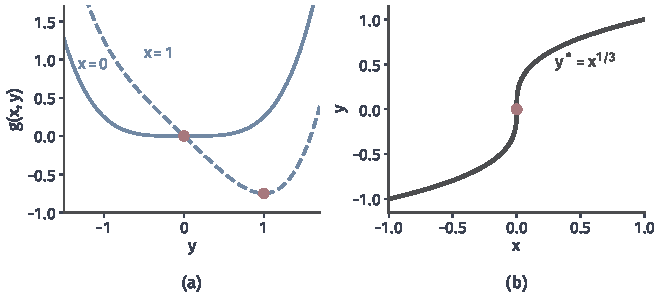
\includegraphics[width=112mm]{figures/05-optimization/07-multiple-criteria-and-nested-optimization/matplotlib/bilevel-singular/figure.pdf}
 \caption{内解唯一但不可微，$g=y^4/4-xy$。(a)$x=0$（实线）的碗底平坦，$H=0$；$x=1$（虚线）的碗底在$y=1$，红点是内解。(b)内解曲线$y^\star=x^{1/3}$连续，红点$x=0$处切线竖直。}
 \label{fig:bilevel-singular}
\end{BookInlineFigure}

\subsection{分支切换}
\label{sec:bilevel-switching}

内层非凸时，几个局部极小点可能并存，谁是全局最优随$\bm{x}$改变。局部分支一直光滑，全局选解却可能在某处跳到另一条分支上。

\paragraph{两个碗交换优劣}
构造一个可以手算的内层，它由两个抛物线取下包络：
\begin{equation}
 g(x,y)=\min\Bigl\{\frac12(y-1-x)^2-x,\ \ \frac12(y+1-x)^2+x\Bigr\}.
 \label{eq:bilevel-two-wells}
\end{equation}

令两式相等并化简，可知两条抛物线始终在$y=0$处相交，那里是两个碗之间的山脊。山脊不在碗底，所以每个碗底附近$g$就是一条光滑的抛物线，定理~\ref{thm:bilevel-local-branch}适用。第一个碗的碗底$y_+(x)=x+1$在$x>-1$时位于山脊右侧，第二个碗的碗底$y_-(x)=x-1$在$x<1$时位于山脊左侧。两个碗底的高度分别是
\[
 g(x,y_+(x))=-x,\qquad g(x,y_-(x))=x.
\]

所以$x>0$时右边的碗更低，$x<0$时左边的碗更低，$x=0$时打平。全局解集是
\[
 S(x)=\begin{cases}
 \{x-1\}, & x<0,\\
 \{-1,\ 1\}, & x=0,\\
 \{x+1\}, & x>0.
 \end{cases}
\]

图~\ref{fig:bilevel-switch-inner}(a)画了三个$x$处的$g$，(b)画了解曲线。全局选解在$x=0$处从下面一条分支跳到上面一条，两条分支本身都连续穿过$x=0$。

\begin{BookInlineFigure}
 \centering
 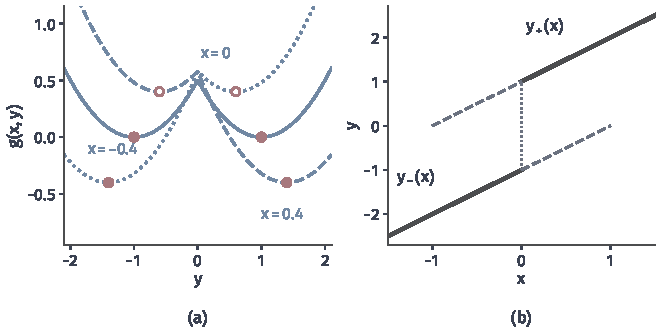
\includegraphics[width=112mm]{figures/05-optimization/07-multiple-criteria-and-nested-optimization/matplotlib/bilevel-switch-inner/figure.pdf}
 \caption{两个内层极小点交换优劣，$g$由式~\eqref{eq:bilevel-two-wells}定义。(a)$x=-0.4,0,0.4$时的$g$，红色实心点是全局极小点，空心点是非全局的局部极小点。(b)深灰粗线是全局内解，灰色虚线是仍为局部极小点、但已不是全局最优的分支延续，点线标出$x=0$处的跳变。}
 \label{fig:bilevel-switch-inner}
\end{BookInlineFigure}

\paragraph{外层目标跟着跳}
取外层目标$F=\frac12(y-\frac12)^2$。沿两条分支的外层值分别是
\[
 \Phi_+(x)=\frac12\Bigl(x+\frac12\Bigr)^2,\qquad\Phi_-(x)=\frac12\Bigl(x-\frac32\Bigr)^2.
\]

全局选解的外层值在$x>0$时是$\Phi_+$，在$x<0$时是$\Phi_-$。在$x=0$处从左极限$9/8$跳到右极限$1/8$，$\Phi$在这里甚至不连续。乐观模型在$x=0$选$y=1$，值为$1/8$；悲观模型选$y=-1$，值为$9/8$。

\paragraph{算法实际追踪的是哪一条}
现在假定外层用梯度下降，内层每次从上一轮的解继续求解。这种\term{热启动}（warm start）使内层一直留在右边的碗里。若沿分支用光滑公式，外层迭代是
\[
 x^{(t+1)}=x^{(t)}-\eta\,\Phi_+'(x^{(t)})=x^{(t)}-\eta\Bigl(x^{(t)}+\frac12\Bigr).
\]

从$x^{(0)}=0.8$出发，取$\eta=0.3$，迭代穿过$x=0$，一路收敛到$x=-\frac12$，此时外层值看上去是$0$。这是图~\ref{fig:bilevel-switch-phi}中的绿色路径。

可是$x=-\frac12$时右边的碗已经不是全局最优了。真正的内解在左边的碗里，$y_-(-\frac12)=-\frac32$，真实的外层值是
\[
 \Phi_-\Bigl(-\frac12\Bigr)=\frac12\Bigl(-\frac12-\frac32\Bigr)^2=2.
\]

算法报告的$0$和真实的$2$之间差了一条红色点线的距离，而算法运行中没有任何量发出警告，因为沿局部分支一切都光滑。

\begin{BookInlineFigure}
 \centering
 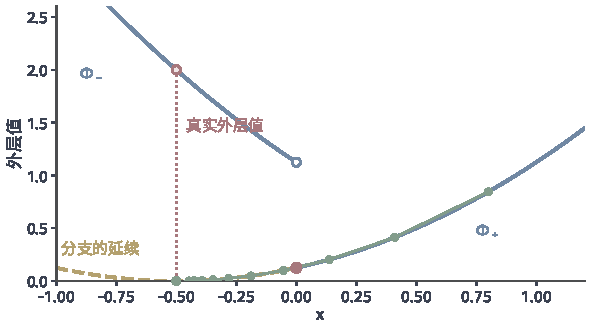
\includegraphics[width=100mm]{figures/05-optimization/07-multiple-criteria-and-nested-optimization/matplotlib/bilevel-switch-phi/figure.pdf}
 \caption{全局选解的外层值在切换点跳变，$F=\frac12(y-\frac12)^2$。蓝线是全局选解的外层值，$x=0$处的空心点是左极限$9/8$，红点是右极限$1/8$，也是乐观模型在$x=0$的值。黄色虚线是分支$\Phi_+$越过切换点后的延续，绿色路径是沿这条分支的外层梯度下降，它停在$x=-1/2$。红色空心点是此处真实的外层值$2$。}
 \label{fig:bilevel-switch-phi}
\end{BookInlineFigure}

表~\ref{tab:bilevel-three-derivatives}分清这里出现的三个“导数”。切换点处不能继续套用同一个光滑公式，这个公式求的是局部分支的导数，在切换点那一边它不再描述全局选解。

\begin{BookInlineTable}
 \centering
 \begin{tabular}{lll}
  \toprule
  对象 & 例中$x=-0.1$处 & 成立范围\\
  \midrule
  局部分支导数$\Phi_+'$ & $0.4$ & 分支存续的区间\\
  全局选解导数$\Phi_-'$ & $-1.6$ & 不含切换点的区间\\
  算法返回的导数 & 取决于碗的选择 & 取决于初值、热启动\\
  \bottomrule
 \end{tabular}
 \caption{分支切换时要区分的三种导数。例中$x=-0.1$时全局内解在左边的碗，热启动的算法却可能仍在右边的碗。}
 \label{tab:bilevel-three-derivatives}
\end{BookInlineTable}
